\documentclass{article}
\usepackage[a0paper,margin=5mm,paper height=1055mm,paper width=610mm]{geometry}
\usepackage{fontspec}
\usepackage{stringstrings}
\usepackage{tikz,pgf}
\usetikzlibrary{intersections,calc}

%% FONTS 0:Interstate, 1:Yanone Kaffeesatz, 2:Fontin
\def\fontCase{2}

\newcommand{\fd}[4]{\newcommand{#1}{\fontspec[#2]{#4}\fontsize{#3}{#3}\selectfont}}
\ifcase\fontCase
	\fd\mainTitleFont{FakeBold=1,FakeStretch=1.06,WordSpace=15,LetterSpace=2}{62pt}{Interstate Thin}
	\fd\signNameFont{FakeBold=2,FakeStretch=1.08,WordSpace=6}{27pt}{Interstate Thin}
	\fd\signDescFont{FakeBold=5,FakeStretch=1.08,WordSpace=2,LetterSpace=2}{13pt}{Interstate Thin}
	\fd\secTitleFont{FakeBold=0.45,FakeStretch=1.09,WordSpace=10,LetterSpace=2}{50pt}{Interstate Thin}
	\fd\bottomTitleFont{FakeBold=1,FakeStretch=1.06,WordSpace=15,LetterSpace=2}{65pt}{Interstate Thin}
	\newcommand{\Tr}[1]{\uppercase{#1}}
	\newcommand{\signNameShift}{0mm}
\or
	% get Kaffeesatz at: http://www.yanone.de/typedesign/kaffeesatz/
	\fd\mainTitleFont{FakeStretch=1,WordSpace=15,LetterSpace=2}{67pt}{Yanone Kaffeesatz Thin}
	\fd\signNameFont{FakeStretch=1,WordSpace=6}{27pt}{Yanone Kaffeesatz Regular}
	\fd\signDescFont{FakeStretch=1,WordSpace=2,LetterSpace=2}{13pt}{Yanone Kaffeesatz Regular}
	\fd\secTitleFont{FakeStretch=1,WordSpace=10,LetterSpace=2}{50pt}{Yanone Kaffeesatz Thin}
	\fd\bottomTitleFont{FakeStretch=1,WordSpace=15,LetterSpace=2}{70pt}{Yanone Kaffeesatz Thin}
	\newcommand{\Tr}[1]{\uppercase{#1}}
	\newcommand{\signNameShift}{0mm}
\or
	% get Fontin at: http://www.josbuivenga.demon.nl/fontin.html
	% get Fontin Sans at: http://www.josbuivenga.demon.nl/fontinsans.html
	% get Delicious at: http://www.josbuivenga.demon.nl/delicious.html
	\fd\mainTitleFont{}{62pt}{Fontin Bold}
	\fd\signNameFont{}{27pt}{Delicious SmallCaps}
	\fd\signDescFont{}{13pt}{Delicious Roman}
	\fd\secTitleFont{}{50pt}{Fontin Sans Regular}
	\fd\bottomTitleFont{}{65pt}{Fontin Bold}
	\newcommand{\Tr}[1]{#1}
	\newcommand{\signNameShift}{-2.5mm}
\fi
%\color{red}


%% POSITIONING
\newcommand{\baselineStart}{-123.5mm}
\newcommand{\baselineSkip}{-89.2mm}
\newcounter{SignColumn}

\newcommand{\firstrow}{
	\path(0,\baselineStart) coordinate(Baseline);
	\foreach \X in {1,...,10} {
		\path
			let \n0={59.5mm} in
			(\n0 * \X - \n0 * 5.5, 0) coordinate(Column\X);
	}
}
\newcommand{\newrow}{
	\path(Baseline) ++(0,\baselineSkip)coordinate(Baseline);
	\setcounter{SignColumn}{0}
}

\newcommand{\bg}[2]{} % debug

\newcommand{\hsign}[3]{%
	\caselower[q]{#2}
	\edef\texname{signs/\thestring.tex}
	%
	\draw
		#3 coordinate(SignHere)
		(SignHere)++(0,#1)node{\begin{tikzpicture}[
			scale=0.75, ultra thick, line cap=round, line join=round
		]
			\input{\texname}
		\end{tikzpicture}}
		;
}
\newcommand{\xsign}[2][0mm]{%
	\stepcounter{SignColumn}
	\edef\columnName{Column\theSignColumn}
	\hsign{#1}{#2}{%
		(\columnName) coordinate(Column)
		(Column |- Baseline)}
}

\newcommand{\sign}[3][\defname]{%
	\def\defname{#2}
	\xsign[40mm]{#2}
	%
	\draw
		(SignHere)node(SignNameNode)[
			anchor=base, align=center, font=\signNameFont
		]{\Tr{#1}}

		(SignNameNode.base)++(0,\signNameShift) node[
			anchor=north, align=center, font=\signDescFont
		]{\Tr{#3}}
		;
}




\begin{document}
\centering
\begin{tikzpicture}
%	\draw(0,0)node[anchor=north]{ 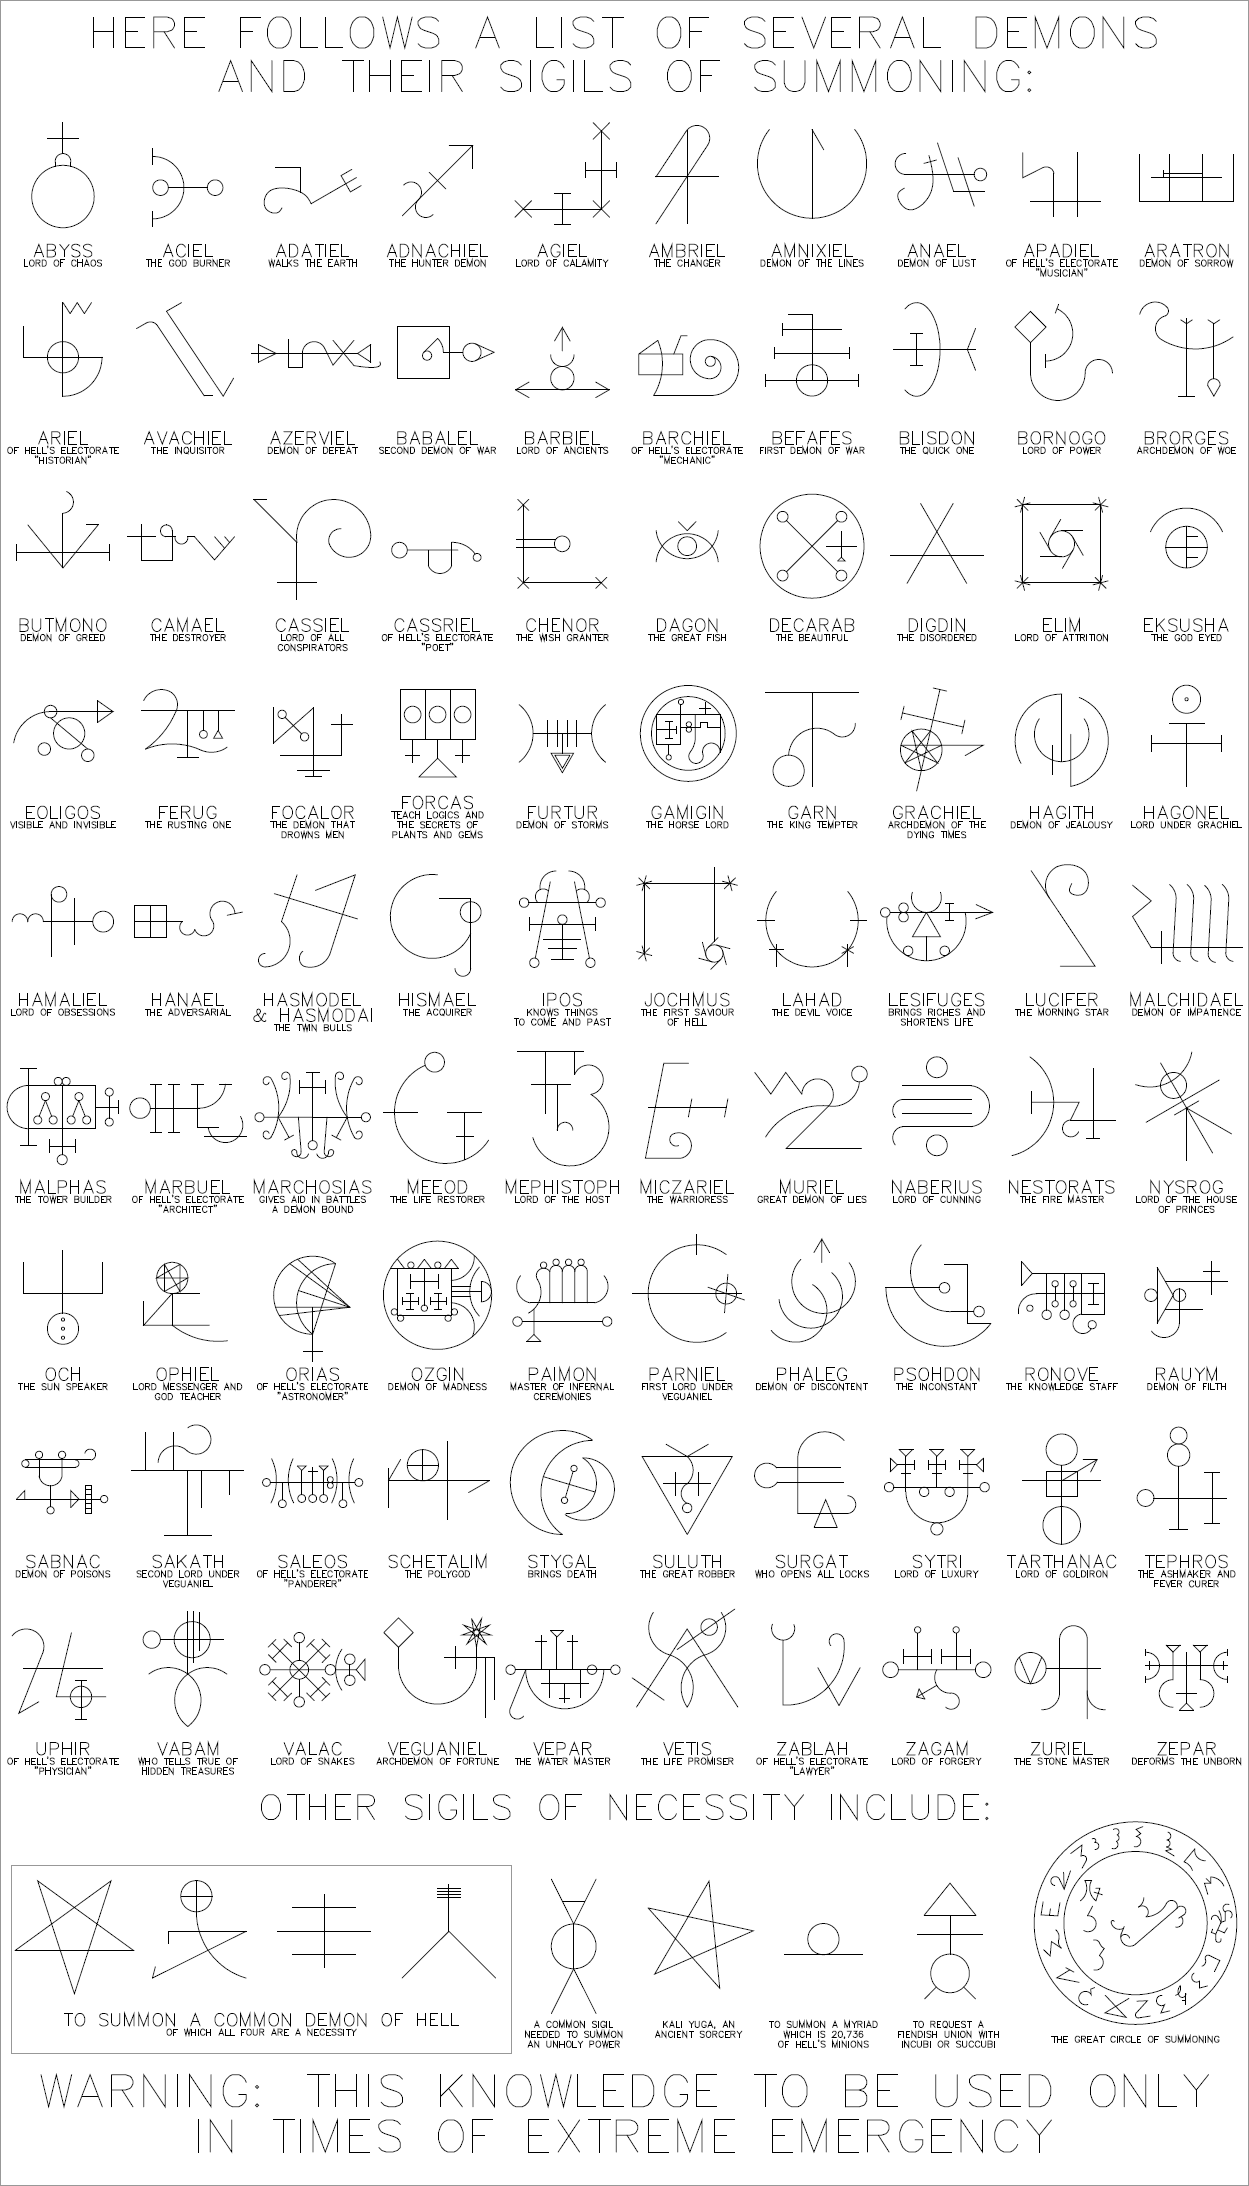
\includegraphics[scale=2.25]{summons-cropped.png} };

	\firstrow
	\sign{Abyss}{Lord of Chaos}
	\sign{Aciel}{The God Burner}
	\sign{Adatiel}{Walks the Earth}
	\sign{Adnachiel}{The Hunter Demon}
	\sign{Agiel}{Lord of Calamity}
	\sign{Ambriel}{The Changer}
	\sign{Amnixiel}{Demon of the Lines}
	\sign{Anael}{Demon of Lust}
	\sign{Apadiel}{of Hell’s electorate\\ “Musician”}
	\sign{Aratron}{Demon of Sorrow}\newrow
	\sign{Ariel}{of Hell’s electorate\\ “Historian”}
	\sign{Avachiel}{The Inquisitor}
	\sign{Azerviel}{Demon of Defeat}
	\sign{Babalel}{Second Demon of War}
	\sign{Barbiel}{Lord of Ancients}
	\sign{Barchiel}{of Hell’s electorate\\ “Mechanic”}
	\sign{Befafes}{First Demon of War}
	\sign{Blisdon}{The Quick One}
	\sign{Bornogo}{Lord of Power}
	\sign{Brorges}{Archdemon of Woe}\newrow
	\sign{Butmono}{Demon of Greed}
	\sign{Camael}{The Destroyer}
	\sign{Cassiel}{Lord of all\\ Conspirators}
	\sign{Cassriel}{of Hell’s Electorate\\ “Poet”}
	\sign{Chenor}{The Wish Granter}
	\sign{Dagon}{The Great Fish}
	\sign{Decarab}{The Beautiful}
	\sign{Digdin}{The Disordered}
	\sign{Elim}{Lord of Attrition}
	\sign{Ekusha}{The God Eyed}\newrow
	\sign{Eoligos}{Visible and Invisible}
	\sign{Ferug}{The Rusting One}
	\sign{Focalor}{The Demon that\\ drowns men}
	\sign{Forcas}{Teach Logics and\\ the secrets of\\ plants and gems}
	\sign{Furtur}{Demon of Storms}
	\sign{Gamigin}{The Horse Lord}
	\sign{Garn}{The King Tempter}
	\sign{Grachiel}{Archdemon of the\\ Dying Times}
	\sign{Hagith}{Demon of Jealousy}
	\sign{Hagonel}{Lord under Grachiel}\newrow
	\sign{Hamaliel}{Lord of Obsessions}
	\sign{Hanael}{The Adversarial}
	\sign[Hasmodel\\ \&~Hasmodai]{hasmodel}{The Twin Bulls}
	\sign{Hismael}{The Acquirer}
	\sign{Ipos}{Knows things\\ to come and past}
	\sign{Jochmus}{The First Saviour\\ of Hell}
	\sign{Lahad}{The Devil Voice}
	\sign{Lesifuges}{Brings riches and\\ shortens life}
	\sign{Lucifer}{The Morning Star}
	\sign{Malchidael}{Demon of Impatience}\newrow
	\sign{Malphas}{The Tower Builder}
	\sign{Marbuel}{of Hell’s electorate\\ “Architect”}
	\sign{Marchosias}{Gives aid in battles\\ A Demon bound}
	\sign{Meeod}{The Life Restorer}
	\sign{Mephistoph}{Lord of the Host}
	\sign{Miczariel}{The Warrioress}
	\sign{Muriel}{Great Demon of Lies}
	\sign{Naberius}{Lord of Cunning}
	\sign{Nestorats}{The Fire Monster}
	\sign{Nysrog}{Lord of the House\\ of Princes}\newrow
	\sign{Och}{The Sun Speaker}
	\sign{Ophiel}{Lord Messenger and\\ God Teacher}
	\sign{Orias}{of Hell’s electorate\\ “Astronomer”}
	\sign{Ozgin}{Demon of Madness}
	\sign{Paimon}{Master of Infernal\\ Ceremonies}
	\sign{Parniel}{First Lord under\\ Veguaniel}
	\sign{Phaleg}{Demon of Discontent}
	\sign{Psohdon}{The Inconstant}
	\sign{Ronove}{The Knowledge Staff}
	\sign{Rauym}{Demon of Filth}\newrow
	\sign{Sabnac}{Demon of Poisons}
	\sign{Sakath}{Second Lord under\\ Veguaniel}
	\sign{Saleos}{of Hell’s electorate\\ “Panderer”}
	\sign{Schetalim}{The Polygod}
	\sign{Stygal}{Brings death}
	\sign{Suluth}{The Great Robber}
	\sign{Surgat}{Who opens all locks}
	\sign{Sytri}{Lord of Luxury}
	\sign{Tarthanac}{Lord of Goldiron}
	\sign{Tephros}{The Ashmaker and\\ Fever Curer}\newrow
	\sign{Uphir}{of Hell’s electorate\\ “Physician”}
	\sign{Vabam}{Who tells true of\\ hidden treasures}
	\sign{Valac}{Lord of Snakes}
	\sign{Veguaniel}{Archdemon of Fortune}
	\sign{Vepar}{The Water Master}
	\sign{Vetis}{The Life Promiser}
	\sign{Zablah}{of Hell’s electorate\\ “Lawyer”}
	\sign{Zagam}{Lord of Forgery}
	\sign{Zuriel}{The Stone Master}
	\sign{Zepar}{Deforms the unborn}

	\tikzset{K/.style={anchor=north, align=center}}

	\draw(0,-8mm)node[K,font=\mainTitleFont]{\Tr{%
		Here follows a list of several Demons\\%
		and their Sigils of Summoning:}};

	\draw(Baseline)++(0,-17mm)++(0,-5mm)node[K,font=\secTitleFont]{\Tr{%
		Other Sigils of necissity include:}};

	\newrow
	% shift baseline up, odd free space:
	\path (Baseline) ++(0,5mm) coordinate(Baseline);

	\xsign{common1}
	\xsign{common2}
	\xsign{common3}
	\xsign{common4}
	\draw ($(Column2)!0.5!(Column3)$) coordinate(Column25)
		(Column25 |- Baseline) ++(0,-40mm) coordinate(B)
		(B) node[K, anchor=south, font=\signNameFont]{\Tr{%
			To summon a common Demon of Hell}}
		(B) node[K, font=\signDescFont]{\Tr{%
			Of which all four are a necessity}};

	\newcommand{\TextHere}{++(0,-36mm)}
	\tikzset{S/.style={K,font=\signDescFont}}

	\xsign{unholy}
	\draw (SignHere)\TextHere node[S]{\Tr{%
		A common Sigil\\%
		needed to summon\\%
		an Unholy Power}};

	\xsign{kaliyuga}
	\draw (SignHere)\TextHere node[S]{\Tr{%
		Kali Yuga, an\\%
		ancient sorcery}};

	\xsign{myriad}
	\draw (SignHere)\TextHere node[S]{\Tr{%
		To summon a Myriad\\%
		which is 20,736\\%
		of Hell's minions}};

	\xsign{union}
	\draw(SignHere)\TextHere node[S]{\Tr{%
		To request a\\%
		fiendish union with\\%
		Incubi or Succubi}};

	\hsign{10mm}{circle}{%
		($(Column9)!0.5!(Column10)$) coordinate(Column95)
		(Column95 |- Baseline)}
	\draw(SignHere)++(0,-43mm) node[S]{\Tr{%
		The Great Circle of Summoning}};

	\draw(Baseline)++(0,-61mm)++(0,-5mm)node[K,font=\bottomTitleFont]{\Tr{%
		Warning: This knowledge to be used only\\%
		in times of extreme emergency}};
	;
\end{tikzpicture}
\end{document}
